\documentclass[12pt]{article}
\usepackage{graphicx}
\usepackage[margin=0.8in]{geometry}
\begin{document}
{\bf Names:} Jack Bracewell, Milan Misak, Craig Ellis \\
{\bf Usernames:} jb2910, mm5510, ce710 \\
{\bf Group Number: 28}  \\ \\

\section*{Assignment 4: Case Based Reasoning}

\subsubsection*{How did you solve the problem of finding two or more best matches with different labels in function RETRIEVE?}

In \emph{retrieve} we iterate over all the cases and calculate the similarity of each case and the one passed into the function. We store the value of the highest similarity we have found so far, and an array of cases which had that similarity. Once we have iterated through all of the cases, we calculate the sum of the typicalities of the cases in our array, for each emotion. We return the first case whose emotion is the same as the one with the highest total. \\

\subsubsection*{Discuss what happens if you try to add a case to CBR system that is already there (either initialisation phase or when you call the retain function? How did you deal with this issue?}

We just increment the typicality of the case that is already in the CBR system and discard the new case. 

\subsubsection*{Compare the different similarity measures you have used (at least three). What are the advantages/disadvantages of each measure?}

The first similarity measure we used was the size of the intersection of 2 AU vectors, normalised. This method was quite quick but only resulted in a classification rate of 73.2. \\ 

We also used the Jaccard Index and Dice coefficient (used to measure the similarity of 2 sets) as measures. These had surprisingly the same $F_1$ measure of 77.5, while still being relatively quick due to not needing to be normalised. \\

The final similarity measure we tried was a normalised Levenshtein Distance between 2 problems. It is normally used to compare strings to provide correction suggestions in spellcheckers, but because the AU Vector always had the same ordering we could still use it to compare their similarity. It was so slow that we do not have cross validation results for it using our K-NN method. For comparison, Dice's classification rate using our faster system (which involved calculating average AU vectors for each category, so only 6 similarities needed to be calculated as opposed to one for every case) was: 42.2, Jaccard's: 50.5, and Levenshtein was 43.3. The Cross Validation for Levenshtein took minutes compared to a couple of seconds for the other similarity measures.  \\

In the end, we used the Dice coefficient with 3-nearest neighbours. Jaccard perfomed a very small amount better (provided an $F_1$ measure of 0.2 higher), but took more than 1.25 times as much time, so we decided that the trade-off was worth it. \\ \\

\subsubsection*{Describe how you initialise your CBR system.}

Our CBR system is fairly simple, as it only consists of a cell array of cases. To initialise it we iterate over examples in the given clean data and create a case for each example on the fly. For every case we check if the CBR system already contains an equal case, and if so then we increment typicality of the already stored case, otherwise we add the new case to the CBR system.

\subsubsection*{CBR belongs to a specific class of learning algorithms?! How are these algorithms called and what are the differences with other learning algorithms, like neural networks and decision trees?}
%TODO: that first sentence isn't even a question... I've put an exclamation mark there to see if anyone notices. Good job; I noticed

Online learning algorithms. The difference is that for online algorithms the learning never ends. Their performance should be continually improved with every new case they encounter. Offline learning algorithms do not continue learning once the training is completed.

\subsection*{Implementation details}
\begin{itemize}
  \item RETRIEVE:
    We Cycle through all the cases in the structure, picking the cases with the 3 highest similarities to the case we are attempting to classify (3-NN). If there are more than 3 with the highest similarity then they are all included in the "voting", and not discarded. For example, case one has a similarity of 79, case two has 78, and cases three and four both have similarities of 77. We cannot decide which of cases three and four to keep in the 'top three', so we include both.
  \item REUSE:
    We simply assign the solution value from the retrieved case to the case we are classifying.
  \item RETAIN:
    A new case is made with the corresponding AU Vector and solution that was found. The weight is a value used for calculating similarity, and is set to 0.8 for every new case, because that is roughly the classification rate, ie - how much we should trust the prediction, compared to the training data which we know is correct.
  \item CBR cases:
    Each case has an AUVector, a solution, and a typicality value, the use of which is explained previously.
\end{itemize}

\subsection*{Evaluation results}

\begin{table}
\centering
\begin{tabular}{r r | r r r r r r}
\multicolumn{8}{c}{Predicted class} \\
&  & Anger & Disgust & Fear & Happiness & Sadness & Surprise \\
\hline
 & Anger            & 9.6 & 1.3  & 0.6 & 0.9  & 0.5 & 0.3  \\
 & Disgust          & 1.7 & 14.9 & 0.3 & 1.7  & 0.8 & 0.4  \\
Actual class & Fear & 1.0 & 0.1  & 8.2 & 0.4  & 0.1 & 2.1  \\
 & Happiness        & 0.1 & 0.8  & 0.2 & 19.9 & 0.1 & 0.5  \\
 & Sadness          & 2.4 & 1.8  & 0.9 & 0.9  & 6.6 & 0.6  \\
 & Surprise         & 0.1 & 0.3  & 0.7 & 0.4  & 0.1 & 19.1 \\
\end{tabular} 
\caption{Confusion matrix}
\end{table}

\begin{table}
\centering
\begin{tabular}{l | r r}
Emotion & Recall rate (\%) & Precision rate (\%) \\
\hline
Anger     & 72.7273 & 64.4295 \\
Disgust   & 75.2525 & 77.6042 \\
Fear      & 68.9076 & 75.2294 \\
Happiness & 92.1296 & 82.2314 \\
Sadness   & 50.0000 & 80.4878 \\
Surprise  & 92.2705 & 83.0435 \\
\end{tabular}
\caption{Recall and precision rates}
\end{table}

\begin{table}
\centering
\begin{tabular}{l | r}
Emotion & \( F_1 \) measure \\
\hline
Anger     & 68.3274 \\
Disgust   & 76.4103 \\
Fear      & 71.9298 \\
Happiness & 86.8996 \\
Sadness   & 61.6822 \\
Surprise  & 87.4142 \\
\end{tabular}
\caption{F1 measures}
\end{table}

Average classification rate = 0.7830 \\ \\

Confusion matrix: the confusion matrix shows that our cbr performs fairly well. Sadness, however, is often misclassified as other classes, specifically Anger. Anger itself is chosen fairly often to classify any case (meaning many emotions are often mistaken for anger). \\
Classification rate: Not as good as some previous classification methods (eg. neural networks), it is still always over 70\%, and almost always above 75\%, after some tweaking of the k nearest neighbours and the weight given to classified cases, which is a reasonable success rate. \\
Recall/Precision rate: These are fairly high for most emotions, with just a few cases bringing the average right down. Sadness, for example, was only recognised correctly 50\% of the time, and fear only 68\%. As stated before, anger was often used incorrectly as a classification, resulting in its low precision rate. The $F_1$ measure confirms this, with all emotions but sandness and anger scoring above 70\%. \\

\newpage
\subsection*{Code Flowchart}

TODO
%\begin{center}
%  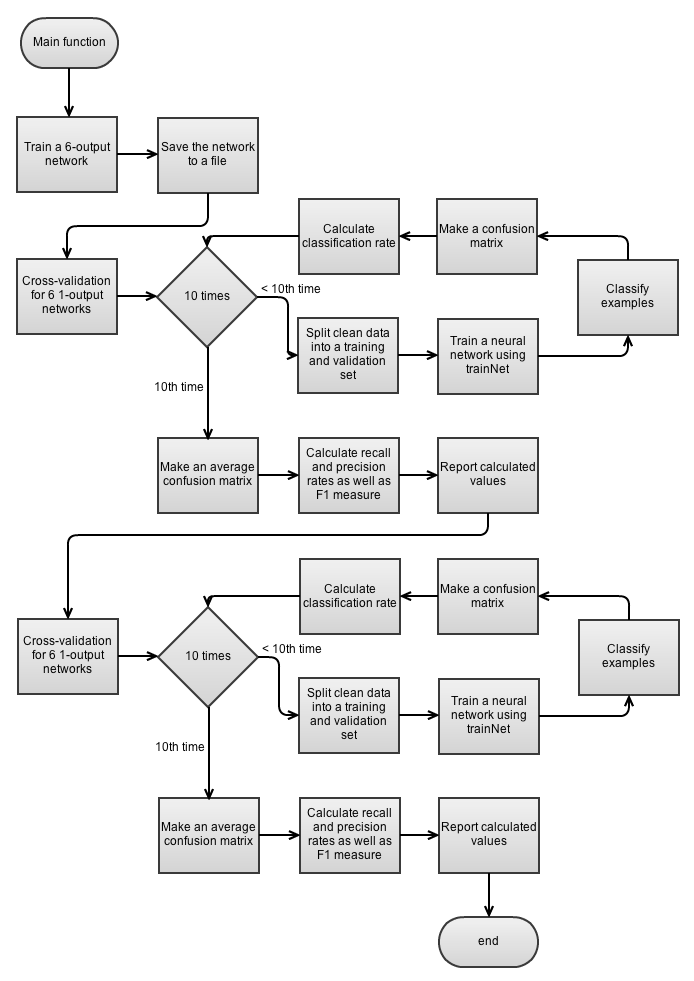
\includegraphics[scale=0.7]{report-images/main.png}
%\end{center}



\end{document}
